\chapter{Neuronale Netze in Tensorflow}
Neuronale Netze sind das am h\"aufigsten benutzte Werkzeug in Tensorflow. Im Folgenden werden die Grundlagen f\"ur Neuronale Netze vorgestellt, sowie deren Umsetzung in Tensorflow. Diverse Codeauschnitte in diesem und alle nachfolgenden Kapitel sind Implementierungen in der Programmiersprache Python.

\section{Feedforwardnetzwerk}
Die h\"aufigste in Tensorflow implementierte Version Neuronaler Netze ist das Feed Forward Netz. Diese werden auch am h\"aufigsten f\"ur Deep Learning verwendet.\footnote{\cite{Goodfellow} S.168}
Ein Feed Forward Netz besteht aus einer Eingabeschicht, einer Ausgabeschicht und n versteckten Schichten dazwischen.
\begin{figure}[!htp]
	\setlength{\unitlength}{1cm}
	\centering
	\begin{picture}(4,3.5)
	\label{FeedForward}
	
	\put(-0.2,0.5){\textcolor{blue}{$w_{1,1}$}}
	\put(1.35,0.26){\textcolor{blue}{$w_{2,1}$}}
	\put(2.8,0.2){\textcolor{blue}{$w_{n,1}$}}
	\put(4.1,0.6){\textcolor{green}{$w_{n,{m_1}}$}}
	
	\put(0.53,-0.1){$x_1$}
	\put(2.05,-0.1){$x_2$}
	\put(3.54,-0.1){$x_n$}
	\put(4.5,-0.1){\textbf{Inputschicht}}
	
	\put(0.75,0){\circle{0.5}}
	\put(2.25,0){\circle{0.5}}
	\put(3.75,0){\circle{0.5}}
	
	\put(0,1.5){\circle{0.5}}
	\put(1.5,1.5){\circle{0.5}}
	\put(3,1.5){\circle{0.5}}
	\put(4.5,1.5){\circle{0.5}}
	\put(5.25,1.35){\textbf{Versteckte Schicht}}
	
	\put(1.5,3){\circle{0.5}}
	\put(1.3,2.9){$o_1$}
	\put(3,3){\circle{0.5}}
	\put(2.8,2.9){$o_2$}
	\put(4.05,2.85){\textbf{Outputschicht}}
	
	\put(0.75,0.25){\textcolor{blue}{\line(-3,5){0.63}}}
	\put(0.75,0.25){\line(3,5){0.63}}
	\put(0.75,0.25){\line(2,1){2.1}}
	\put(0.75,0.25){\line(3,1){3.5}}
	
	\put(2.25,0.25){\line(-3,5){0.63}}
	\put(2.25,0.25){\line(3,5){0.63}}
	\put(2.25,0.25){\line(2,1){2.1}}
	\put(2.25,0.25){\textcolor{blue}{\line(-5,3){2}}}
	
	\put(3.75,0.25){\line(-3,5){0.63}}
	\put(3.75,0.25){\textcolor{green}{\line(3,5){0.63}}}
	\put(3.75,0.25){\textcolor{blue}{\line(-3,1){3.5}}}
	\put(3.75,0.25){\line(-5,3){2}}
	
	\put(0,1.75){\line(1,1){1.25}}
	\put(0,1.75){\line(2,1){2.77}}
	
	\put(1.5,1.75){\line(1,1){1.25}}
	\put(1.5,1.75){\line(0,1){1}}
	
	\put(3,1.75){\line(-1,1){1.25}}
	\put(3,1.75){\line(0,1){1}}
	
	\put(4.5,1.75){\line(-1,1){1.25}}
	\put(4.5,1.75){\line(-2,1){2.77}}

	\end{picture}
	\caption{Feed Forward Netz}
\end{figure}
Hierbei ist jedes Neuron mit jedem Neuron der nachfolgenden Schicht durch Gewichte verbunden.\\
Die Abbildung zeigt beispielhaft ein Feed Forward Netzwerk mit 3 Input-Neuronen in der Eingabeschicht, einer versteckten Schicht mit 4 versteckten Neuronen und einer Ausgabeschicht mit 2 Ausgabe-Neuronen.\footnote{\cite{Bishop1995}s.117}\\
Ein Feed Forward Netzwerk kann beliebig viele versteckten Schichten enthalten, aber nur eine Eingabe und eine Ausgabeschicht. Ebenso kann die Anzahl der Neuronen in den versteckten Schichten frei gew\"ahlt werden. Eine sinnvolle Anzahl von Neuronen in den versteckten Schichten l\"asst sich nur experimentell bestimmen.\footnote{\cite{handson} S.385} Man sollte darauf achten nicht zu wenige Neuronen zu verwenden da sonst die Lernkapazit\"at m\"oglicherwei\ss e zu eingeschr\"ankt ist. Auch zu viele Neuronen k\"onnen problematisch sein, da es sehr lang dauern kann jede der vielen Neuronen zu trainieren und die Effizienz des Netzwerks darunter leidet.\footnote{\cite{Rashid} S.341}\\ Man kann bereits mit einer versteckten Schicht und einer ausreichend gro\ss en Anzahl Neuronen jedes Problem simulieren, tendenziell ist es aber besser die Anzahl der Schichten zu erh\"ohen anstatt die Anzahl der Neuronen pro Schicht.\footnote{\cite{handson} S.384}
\section{Der Input Tensor}
Vektoren und Matrizen werden in Tensorflow als Tensors bezeichnet. Der Input eines Neuronalen Netzes ist ein n-dimensionaler Vektor der f\"ur jedes Input-Neuron einen Wert enth\"alt. Die Anzahl der Input-Neuronen richtet sich nach dem untersuchten Problem. Das Einf\"uhrungsbeispiel f\"ur Tensorflow das in etwa dem $"$Hello World$"$ f\"ur Programmiersprachen entspricht, behandelt ein Klassifikationsproblem.\footnote{\cite{handson} S.124} In diesem Problem sollen mithilfe der MNIST Datenbank die tausende von handgeschriebenen $28 \times 28$ Bilder der Zahlen von 1-9 enth\"alt, das Neuronale Netz lernen handgeschriebene Ziffern zu unterscheiden. F\"ur jedes dieser Bilder hat man entsprechend eine $28 \times 28$ Matrix mit Grauwerten. Mit dem Befehl \lstinline$reshape(-1,..)$ \footnote{\cite{handson} S.99} l\"asst es sich in einen eindimensionalen Vektor mit  $28*28=784$ Input Neuronen verwandeln.\\
Input-Tensore werden in Tensorflow mit Platzhaltern angelegt, da w\"ahrend des Lernprozesses der Inputtensor f\"ur jedes zu lernende Beispiel aktualisiert wird. Um den Platzhalter anzulegen verwendet man den Befehl\begin{lstlisting}
input= tf.placeholder("float",[None,Input_Neuronen])
\end{lstlisting}\footnote{\cite{cookbook} S.218} 
Mit float wird der Datentyp des inputs f\"ur die einzelnen Neuronen gew\"ahlt. Die Variable \lstinline$Input_Neuronen$ gibt die Anzahl der Input Neuronen an. Das None steht f\"ur die Anzahl der Trainingsdaten, die sp\"ater noch dynamisch eingef\"ugt wird. So muss man sich zun\"achst nicht festlegen wie viele Trainingsdaten man benutzen will.\footnote{\cite{handson} S.377}

\section{Gewichte}
Man kann alle Gewichte zwischen Inputschicht und der ersten versteckten Schicht als Gewichtsmatrix \begin{equation}
W\textsuperscript{(1)}:=
\begin{pmatrix}
w_{1,1}\textsuperscript{(1)} & w_{1,2}\textsuperscript{(1)} & \cdots & w_{1,m_1}\textsuperscript{(1)} \\
w_{2,1}\textsuperscript{(1)} & w_{2,2}\textsuperscript{(1)}& \cdots & .\\
w_{3,1}\textsuperscript{(1)} & w_{3,2}\textsuperscript{(1)}& \cdots & .\\
\vdots & \vdots & \vdots & \vdots \\
w_{n,1}\textsuperscript{(1)} & w_{n,2}\textsuperscript{(1)} & \cdots & w_{n,m_1}\textsuperscript{(1)}\\
\end{pmatrix} \end{equation}
auffassen.\\\\
Die Zeilen von $W\textsuperscript{(1)}$ entsprechen allen ausgehenden Verbindungen f\"ur ein Neuron aus der Input-Schicht. Die Spalten entsprechen den eingehenden Verbindungen f\"ur ein Neuron aus der versteckten Schicht. \\\\
Der Tensorflow Befehl um die Gewichte zwischen zwei Schicht zu Initialisieren lautet:\\
\begin{lstlisting}
init = tf.truncated_normal(n_inputs, n_neurons)
W =tf.Variable(init,name="weights")
\end{lstlisting}\footnote{\cite{handson} S.377}
Damit werden die Gewichte mit zuf\"alligen Gewichten belegt und es wird eine Matrix bzw Tensor der Dimension \lstinline$(input_neuronen$$ \times $\lstinline$versteckte_neuronen)$ erzeugt.\\
Um den Output des Neuronalen Netzes zu berechnen f\"uhrt man den Befehl \lstinline$tf.matmul(input,W)$ eine Matrix Multiplikation zwischen Input-Tensor und Gewichtsmatrix durch.\footnote{\cite{handson} S.377}\\
Auf diese Weise bekommt man einen weiteren Tensor der f\"ur jedes versteckte Neuron einen Wert hat. Auf diese Werte wendet man nun eine Aktivierungsfunktion an, das Ergebnis nennt man \textbf{Aktivit\"at}\footnote{\cite{Ertel2013} S.247} der versteckten Schicht. Dieses Verfahren kann man nun f\"ur beliebig viele versteckte Schichten wiederholen, dabei nutzt man die Aktivit\"at und die Gewichtsmatrix f\"ur die zweite versteckte Schicht um eine Matrix Multiplikation durchzuf\"uhren und die Aktivit\"at der n\"achsten Schicht zu bekommen.
\section{Aktivierungsfunktionen}
Aktivierungsfunktionen werden verwendet um den Wertebereich den die Neuronen annehmen k\"onnen einzugrenzen. So liegen manche Aktivierungsfunktionen nur zwischen den Werten $-1$ und $1$ oder bilden alle negative Werte auf Null ab. Exemplarisch werden 3 der beliebtesten Aktivierungsfunktionen beschrieben.
\subsection{Rectified linear unit function}
Eine beliebte M\"oglichkeit ist die Rectified linear unit function, kurz relu.\\
F\"ur relu gilt in der parametrisierten Form\footnote{\cite{Goodfellow}S.174 }
\begin{align*}
\sigma(x)=
\left\{
\begin{array}{l l}
& 0 \quad \text{   falls  } \quad x <= 0  \\ 
& ax \quad \text{   sonst}
\end{array}
\right.
\end{align*}
a ist dabei frei w\"ahlbar und kann an das jeweilige Beispiel angepasst werden. Obwohl die Relufunktion eine sehr einfache fast lineare Funktion ist, erweist sie sich als sehr Leistungsf\"ahig. Sie dient als Standardaktivierungsfunktion, die f\"ur die meisten FeedForward Netzwerke empfohlen wird.\footnote{\cite{Goodfellow}S.175 } In Tensorflow ist die Relu Funktion auf verschiedene Arten implementiert, die oben beschriebene Standard Relu Funktion allerdings nur f\"ur den Parameterwert a=1. Sie wird mit
\begin{lstlisting}
tf.nn.relu(features, name=None)
\end{lstlisting}\footnote{\cite{cookbook}S.58f.} 
eingebunden.
Eine andere in tensorflow verwendete Versionen der relu Funktion ist
\begin{lstlisting}
tf.nn.relu6(features, name=None)
\end{lstlisting}\cite{cookbook}
F\"ur diese gilt:
\begin{align*}
	\sigma(x)=
	\left\{
	\begin{array}{l l}
		& 0 \quad \text{   falls  } \quad x <= 0  \\ 
		& x \quad \text{   falls},\quad 0 < x < 6 \\
		& 6 \quad \text{   sonst}
	\end{array}
	\right.
\end{align*}
Sie kann schneller berechet werden und hat den Vorteil das weder Werte nahe der Null verschwinden, noch die Werte zu gro\ss werden k\"onnen.\cite{cookbook} 
\subsection{Sigmoidfunktion}
Eine andere der Standardaktivierungsfunktionen ist die Sigmoid Funktion. Sie eignet sich gut f\"ur das lernen mittels Backpropagation, welches ein sehr h\"aufig eingesetztes Lernverfahren ist.\footnote{\cite{Rojas1996} S.151f.}\\
Die Sigmoidfunktion hat folgende Form:\cite{Rojas1996}
\begin{equation}
\sigma_c(x)=\frac{1}{1+e^{-cx}}
\end{equation}
In Tensorflow ist sie nur mit dem Parameterwert $c=1$ enthalten.
\begin{figure}[!htp]
	\centering
	\includegraphics[page=2,trim = 6cm 14.2cm 5cm 11cm,clip=true,scale=1.1]{images/BackPropRojas.pdf}
	\caption{Sigmoidfunktion f\"ur c=1 \cite{Rojas1996}}
\end{figure}\\
Der Wertebereich der Sigmoidfunktion liegt zwischen 0 und 1, was sich sehr gut eignet falls die Ausgabewerte des Netzwerks ebenfalls in diesem Bereich liegen. In Tensorflow ist sie mit dem Befehl \lstinline$tf.sigmoid(x, name=None)$\footnote{\cite{building}S.175}
definiert.
\subsection{Tangenshyperbolicus}
Der Tangenshyperbolicus ist definiert als\footnote{\cite{Bishop1995}S.127}
\begin{equation}
tanh(x)=\frac{e^x - e^{-x}}{e^x + e^{-x}}.
\end{equation}
Die Ableitungen der Sigmoidfunktion und des Tangenshyperbolicus sind leicht zu berechnen, weshalb sie sich gut zur Berechnung des Gradienten der Fehlerfunktion eignen.
\begin{figure}[!htp]
	\includegraphics[page=3,trim = 10.3cm 22cm 5cm 4.7cm,clip=true,scale=1.4]{images/BackPropRojas.pdf}
	\centering
	\caption{Graph des Tangenshyperbolicus \cite{Rojas1996}}
\end{figure}\\
Wie in der Abbildung ersichtlich wird, befindet sich der Wertebereich des Tangenshyperbolicus im Intervall von [-1,1]. Es wird mit \lstinline$f.tanh(x, name=None)$\footnote{\cite{building}S.175} aufgerufen und eignet sich besonders gut, wenn man in den Lernbeispielen auch negative Zahlen ber\"ucksichtigen will.
\section{Kostenfunktionen}
Kosten- oder Fehlerfunktionen sind ein Ma\ss daf\"ur wie gut ein \gls{NN} lernt. Es stellt eine berechenbare Formel bereit, die den durch das Netz berechneten Output f\"ur ein Trainingsbeispiel mit dem zu lernenden Output vergleicht. Au\ss erdem werden sie f\"ur das lernen des \gls{NN} ben\"otigt, da aus den Ableitungen der jeweiligen Kostenfunktion f\"ur das zugeh\"orige Gewicht die neuen Gewichte gebildet werden.\footnote{\cite{Goodfellow}S.177f.}
\subsection{MSE}
Eine m\"ogliche Kostenfunktion ist der Mean Squared Error, kurz MSE.
\begin{equation}
MSE=\frac{1}{N}\sum_{i=1}^{N} (\^{o}_i-o_i)^2.
\end{equation}\footnote{\cite{Rojas1996}S.156}
$\^{o}$ steht f\"ur den gew\"unschten Output und $o$ f\"ur den vom Netz f\"ur den zugeh\"origen Input Vektor generierten Output.\\
Der MSE wird mit  \lstinline$Kosten=tf.losses.mean_squared_error(labels,predictions)$\footnote{\cite{cookbook}S.94f.} eingebunden und summiert die Quadrate der Abweichungen auf, d.h. je geringer der MSE wird, desto genauer hat das Netz die Trainingsdaten gelernt.
\subsection{cross entropy}
Eine andere M\"oglichkeit ist die sogenannte Cross Entropy Funktion.\footnote{\cite{Nielsen}}
\begin{equation}
CE= - \frac{1}{N} \sum_{i=1}^{N}\^{o}_i \ln o_i + (1- \^{o}_i) \ln (1-o_i)
\end{equation}
Der Vorteil der cross entropy Funktion besteht daran, dass sie je schneller lernt je gr\"o\ss er der anf\"angliche Fehler ist. F\"angt man also bei sehr ung\"unstig gew\"ahlten zuf\"alligen Gewichten mit dem Lernprozess an, wird cross entropy schneller bessere Ergebnisse liefern als der MSE.\footnote{\cite{Nielsen}} Welche man letztendlich verwendet h\"angt vom zugrunde liegenden Problem ab.\\
Cross entropy wird in Tensorflow mit dem Befehl 
\begin{lstlisting}
Kosten=tf.nn.softmax_cross_entropy_with_logits()
\end{lstlisting}verwendet.\footnote{\cite{cookbook}S.88}
\section{Lernprozess}
Damit das Netz lernt m\"ussen St\"uck f\"ur St\"uck die Gewichte angepasst werden. Zu diesem Zweck berechnet man die Ableitung der Kostenfunktion und benutzt sie um die Gewichte abzu\"andern. Dieses Verfahren wird $"$Backpropagation of Error$"$ mittels $"$Gradient Descent$"$ - dem Gradientabstiegsverfahren genannt.\\
Das Update der Gewichte funktioniert nach folgender Regel:\footnote{\cite{Rojas1996}S.157}
\begin{equation}
w_{i,j}=w_{i,j}-\frac{\partial Kosten }{\partial w_{i,j}}\eta,
\end{equation}
wobei $\eta$ die Lernrate darstellt. Diese ist frei w\"ahlbar, \"ublicherweise liegt sie im Bereich von 0.01 und 0.5.\\
Die optimale Lernrate f\"ur das gegebene Problem muss experimentell bestimmt werden, da man dazu im Vorfeld keine genauen Vorhersagen machen kann.
Trainiert wird das Netzwerk letztendlich mit dem Befehl \lstinline$tf.train.GradientDescentOptimizer(Lernrate).minimize(Kosten)$\footnote{\cite{building}S.156}